\documentclass[10pt,twocolumn,letterpaper]{article}

\usepackage{dependable_dnn}
\usepackage{times}
\usepackage{epsfig}
\usepackage{graphicx}
\usepackage{amsmath}
\usepackage{amssymb}
\usepackage{subfigure}
\usepackage[table, dvipsnames]{xcolor}

% Include other packages here, before hyperref.

% If you comment hyperref and then uncomment it, you should delete
% egpaper.aux before re-running latex.  (Or just hit 'q' on the first latex
% run, let it finish, and you should be clear).
\usepackage[pagebackref=true,breaklinks=true,letterpaper=true,colorlinks,bookmarks=false]{hyperref}

\iccvfinalcopy % *** Uncomment this line for the final submission

\def\iccvPaperID{} % *** Enter the Paper ID here
\def\httilde{\mbox{\tt\raisebox{-.5ex}{\symbol{126}}}}

% Pages are numbered in submission mode, and unnumbered in camera-ready
\ificcvfinal\pagestyle{empty}\fi

\begin{document}

%%%%%%%%% TITLE - PLEASE UPDATE
\title{FastNeRF: High-Fidelity Neural Rendering at 200FPS\\ {\rm {\normalsize Seungmin Lee (profile2697@gmail.com; 2020-20866), \\Dept. of Electrical and Computer Engineering, Seoul National University}}}   % **** Enter the paper title and student information here

\maketitle
\thispagestyle{empty}

\section{Introduction and Motivation}
Recent Neural Radiance Fields (NeRF) have demonstrated that neural networks can encode information about a complicated 3D scene and utilize the information to render photorealistic scenes from novel viewpoints. However, NeRF requires too many computations and resources. So, it is hard to use NeRF in real-time rendering. To alleviate the problem, the authors propose caching NeRF's inputs and outputs. However, since NeRF has an extensive input range, naive caching is impossible. Therefore, for the feasible caching, the authors decompose NeRF function, which takes input sized $\mathbb{R}^5$, to two functions that take inputs sized $\mathbb{R}^3$ and $\mathbb{R}^2$, respectively.

\section{Method}
\subsection{NeRF}
NeRF's function takes a 3D position $\mathbf{p} \in \mathbb{R}^3$ and a ray direction $\mathbf{d} \in \mathbb{R}^2$ and maps them to a RGB color value $\{\mathbf{r}, \mathbf{g}, \mathbf{b}\} \in \mathbb{R}^3$ and a transparency $\mathbf{\sigma}$. Therefore has the following form:
\begin{align*}
	\mathcal{F}_{NeRF}: (\mathbf{p}, \mathbf{d}) \rightarrow (\{\mathbf{r}, \mathbf{g}, \mathbf{b}\}, \mathbf{\sigma})
\end{align*}
where $\mathcal{F}_{NeRF}$ is implemented using a neural network.

To render a scene from a new viewpoint, we should call NeRF's function multiple times while changing the input positions for a given ray direction. Since the function is a neural network that requires tons of computations, the rendering process is prolonged. To speed up, we need to cache the function's inputs and outputs while the caching is infeasible because the possible range of input values is too extensive ($\mathcal{R}^5$).

\subsection{FastNeRF}
To realize a feasible cache, the authors propose to decompose the NeRF function into two separate parts that take inputs sized $\mathcal{R}^3$ and $\mathcal{R}^2$, based on spherical harmonics~\cite{SH1, SH2}.

Therefore, FastNeRF has two functions that has the following forms:
\begin{align*}
	\mathcal{F}_{pos}&: \mathbf{p} \rightarrow (\{\mathbf{u}, \mathbf{v}, \mathbf{w}\}, \mathbf{\sigma})\\
	\mathcal{F}_{dir}&: \mathbf{d} \rightarrow \mathbf{\beta}
\end{align*}
where $\mathbf{u}$, $\mathbf{v}$, $\mathbf{w}$, and $\mathbf{\beta}$ have $\mathbb{R}^D$.
The final $\{\mathbf{r}, \mathbf{g}, \mathbf{b}\}$ is calculated using the following equation:
\begin{align*}
	\{\mathbf{r}, \mathbf{g}, \mathbf{b}\} = \mathbf{\beta}^{\intercal} \cdot \{\mathbf{u}, \mathbf{v}, \mathbf{w}\}
\end{align*}
where $\cdot$ denotes the dot product (Fig.~\ref{fig:imgs}).
By doing so, we can reduce the memory complexity from $O(k^3l^2)$ to $O(k^3 * (1 + D^3) + l^2 * D)$, where $k$ is the number of possible values of $\mathbf{p}$'s each dimension, and $l$ is that of $\mathbf{d}$.

\begin{figure}[t]
	\centering
	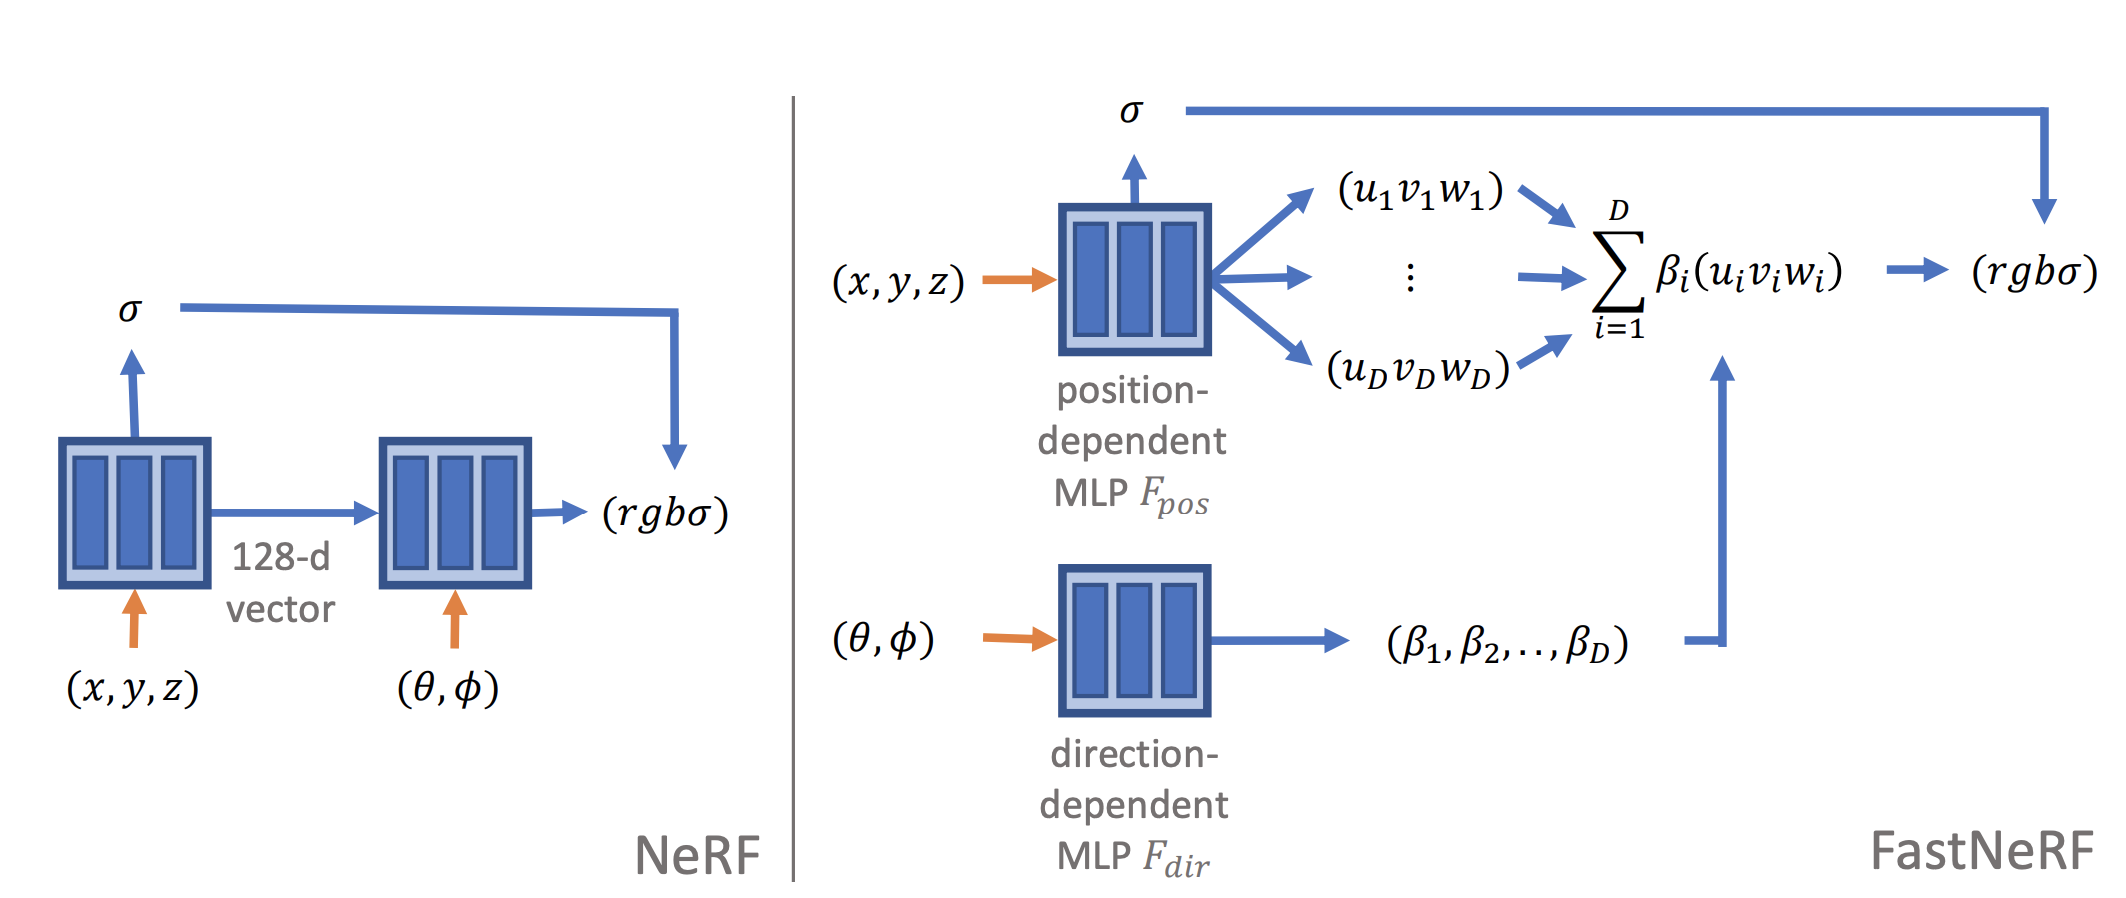
\includegraphics[width=8cm]{assets/FastNeRF.png}
	\caption{The Comparison between NeRF and FastNeRF.}
	\label{fig:imgs}
\end{figure}

\section{Results}
The experimental results show that FastNeRF is about 3000 times faster than the original algorithm while preserving rendering quality. Moreover, the authors' proposed method is the first NeRF-based algorithm to render high-resolution photorealistic images using high-end consumer GPUs.

\section{Personal Note}
The paper improves NeRF's FPS thousands of times. Furthermore, I think the proposed method is simple, effective, and has a solid base in the graphics field. Therefore, the paper seems valuable and practical.

{\small
\bibliographystyle{ieee}
\bibliography{egbib}
}

\end{document}
